\documentclass[tikz,border=10pt]{standalone}
\usepackage{amsmath}
\usepackage{tikz}
\usetikzlibrary{shapes,arrows,positioning,fit,calc,shadows,decorations.pathreplacing}

\begin{document}
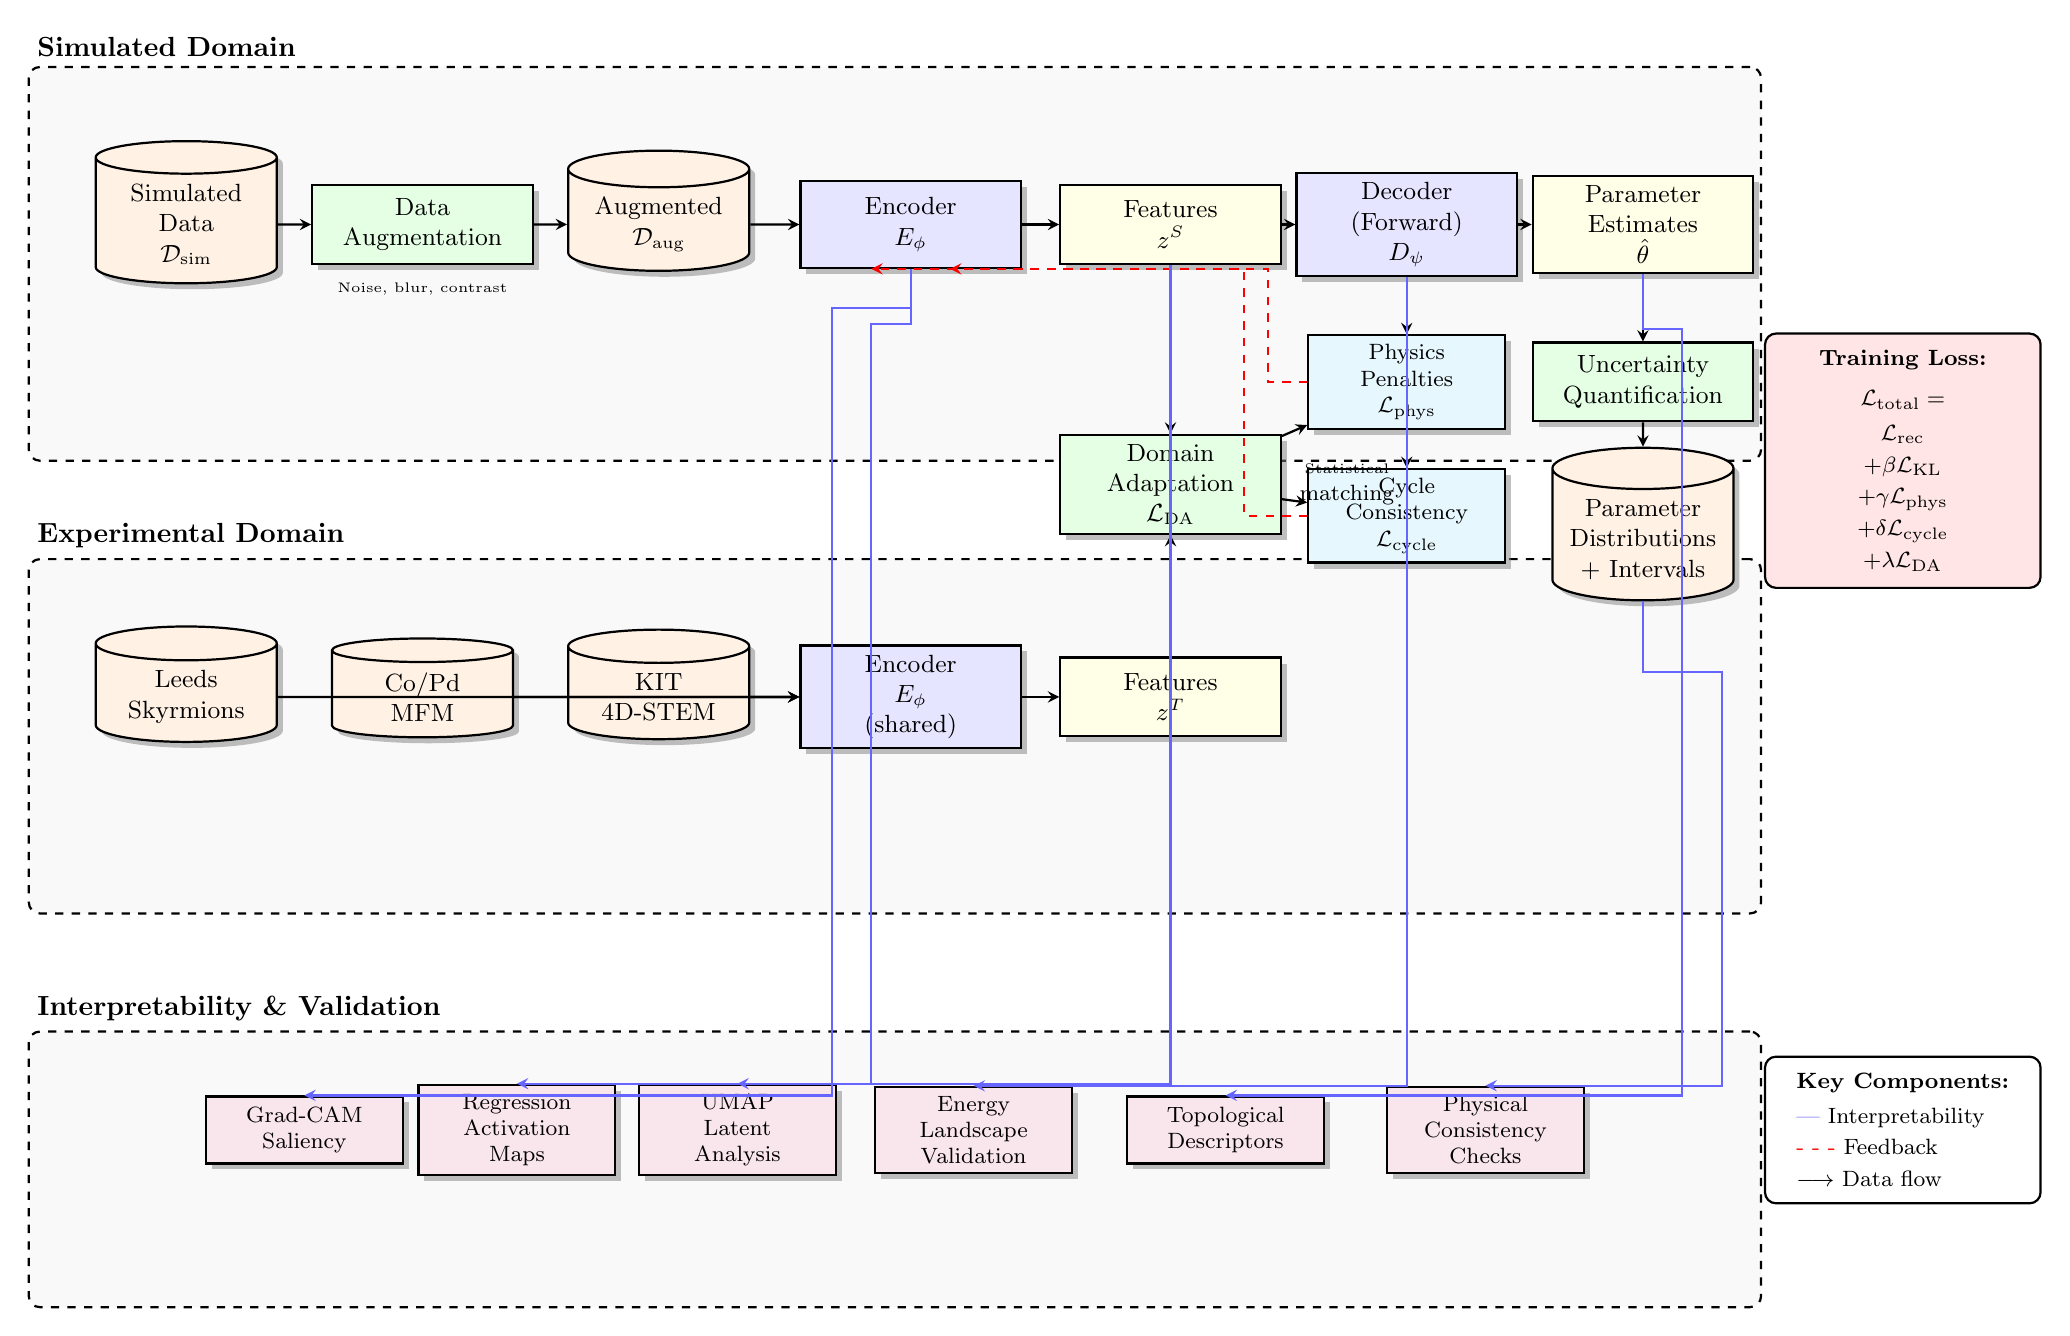
\begin{tikzpicture}[
    node distance=2cm and 2.2cm,
    box/.style={rectangle, draw, thick, fill=blue!10, minimum width=2.8cm, minimum height=1.1cm, align=center, drop shadow, font=\small},
    process/.style={rectangle, draw, thick, fill=green!10, minimum width=2.8cm, minimum height=1cm, align=center, drop shadow, font=\small},
    data/.style={cylinder, draw, thick, fill=orange!10, minimum width=2.3cm, minimum height=1.1cm, align=center, drop shadow, shape border rotate=90, aspect=0.25, font=\small},
    arrow/.style={->, >=stealth, thick},
    dashedarrow/.style={->, >=stealth, thick, dashed, red},
    label/.style={font=\footnotesize, align=center},
    highlight/.style={rectangle, draw, thick, fill=yellow!10, minimum width=2.8cm, minimum height=1cm, align=center, drop shadow, font=\small},
    domainbox/.style={rectangle, draw, dashed, thick, fill=gray!5, rounded corners, inner sep=10pt},
    interpret/.style={rectangle, draw, thick, fill=purple!10, minimum width=2.5cm, minimum height=0.85cm, align=center, drop shadow, font=\footnotesize},
    physbox/.style={rectangle, draw, thick, fill=cyan!10, minimum width=2.5cm, minimum height=0.85cm, align=center, drop shadow, font=\footnotesize}
]

% Main domains
\node[domainbox, minimum width=22cm, minimum height=5cm] (sim_domain) at (0,5) {};
\node[above right, font=\bfseries] at (sim_domain.north west) {Simulated Domain};

\node[domainbox, minimum width=22cm, minimum height=4.5cm] (exp_domain) at (0,-1) {};
\node[above right, font=\bfseries] at (exp_domain.north west) {Experimental Domain};

% ==================== TOP ROW: SIMULATED DATA FLOW ====================
\node[data] (sim_data) at (-9,5.5) {Simulated\\Data\\$\mathcal{D}_{\text{sim}}$};
\node[process] (augment) at (-6,5.5) {Data\\Augmentation};
\node[data] (aug_data) at (-3,5.5) {Augmented\\$\mathcal{D}_{\text{aug}}$};

% Encoder
\node[box] (encoder_s) at (0.2,5.5) {Encoder\\$E_\phi$};
\node[highlight] (features_s) at (3.5,5.5) {Features\\$z^S$};

% Decoder (Forward Model)
\node[box] (decoder) at (6.5,5.5) {Decoder\\(Forward)\\$D_\psi$};
\node[highlight] (params_pred) at (9.5,5.5) {Parameter\\Estimates\\$\hat{\theta}$};

% ==================== BOTTOM ROW: EXPERIMENTAL DATA FLOW ====================
\node[data] (leeds) at (-9,-0.5) {Leeds\\Skyrmions};
\node[data] (mfm) at (-6,-0.5) {Co/Pd\\MFM};
\node[data] (stem) at (-3,-0.5) {KIT\\4D-STEM};

\node[box] (encoder_t) at (0.2,-0.5) {Encoder\\$E_\phi$\\(shared)};
\node[highlight] (features_t) at (3.5,-0.5) {Features\\$z^T$};

% Domain Adaptation
\node[process] (da_align) at (3.5,2.2) {Domain\\Adaptation\\$\mathcal{L}_{\text{DA}}$};

% ==================== PHYSICS CONSTRAINTS (RIGHT SIDE) ====================
\node[physbox] (physics1) at (6.5,3.5) {Physics\\Penalties\\$\mathcal{L}_{\text{phys}}$};
\node[physbox] (cycle) at (6.5,1.8) {Cycle\\Consistency\\$\mathcal{L}_{\text{cycle}}$};

% ==================== UNCERTAINTY QUANTIFICATION (FAR RIGHT) ====================
\node[process] (uncertainty) at (9.5,3.5) {Uncertainty\\Quantification};
\node[data] (output) at (9.5,1.5) {Parameter\\Distributions\\+ Intervals};

% ==================== INTERPRETABILITY LAYER (BOTTOM) ====================
\node[domainbox, minimum width=22cm, minimum height=3.5cm] (interp_domain) at (0,-6.5) {};
\node[above right, font=\bfseries] at (interp_domain.north west) {Interpretability \& Validation};

\node[interpret] (gradcam) at (-7.5,-6) {Grad-CAM\\Saliency};
\node[interpret] (rams) at (-4.8,-6) {Regression\\Activation\\Maps};
\node[interpret] (umap) at (-2,-6) {UMAP\\Latent\\Analysis};

\node[interpret] (energy) at (1,-6) {Energy\\Landscape\\Validation};
\node[interpret] (topology) at (4.2,-6) {Topological\\Descriptors};
\node[interpret] (physical) at (7.5,-6) {Physical\\Consistency\\Checks};

% ==================== ARROWS: SIMULATED FLOW ====================
\draw[arrow] (sim_data) -- (augment);
\draw[arrow] (augment) -- (aug_data);
\draw[arrow] (aug_data) -- (encoder_s);
\draw[arrow] (encoder_s) -- (features_s);
\draw[arrow] (features_s) -- (decoder);
\draw[arrow] (decoder) -- (params_pred);

% ==================== ARROWS: EXPERIMENTAL FLOW ====================
\draw[arrow] (leeds) -- (encoder_t);
\draw[arrow] (mfm) -- (encoder_t);
\draw[arrow] (stem) -- (encoder_t);
\draw[arrow] (encoder_t) -- (features_t);

% ==================== ARROWS: DOMAIN ADAPTATION ====================
\draw[arrow] (features_s) -- (da_align);
\draw[arrow] (features_t) -- (da_align);

% ==================== ARROWS: PHYSICS & CYCLE ====================
\draw[arrow] (da_align) -- (physics1);
\draw[arrow] (da_align) -- (cycle);
\draw[arrow] (decoder) -- (physics1);
\draw[arrow] (decoder) -- (cycle);

% Feedback arrows - routing around blocks
\draw[dashedarrow] (physics1.west) -- ++(-0.5,0) |- ($(encoder_s.south) + (-0.5,0)$);
\draw[dashedarrow] (cycle.west) -- ++(-0.8,0) |- ($(encoder_s.south) + (0.5,0)$);

% ==================== ARROWS: UNCERTAINTY ====================
\draw[arrow] (params_pred) -- (uncertainty);
\draw[arrow] (uncertainty) -- (output);

% ==================== ARROWS: INTERPRETABILITY ====================
% Route these carefully to avoid overlapping with middle blocks
\draw[arrow, blue!60] (encoder_s.south) -- ++(0,-0.5) -- ++(-1,0) |- (gradcam.north);
\draw[arrow, blue!60] (encoder_s.south) -- ++(0,-0.7) -- ++(-0.5,0) |- (rams.north);
\draw[arrow, blue!60] (features_s.south) -- ++(0,-0.9) |- (umap.north);

\draw[arrow, blue!60] (decoder.south) -- ++(0,-0.5) |- (energy.north);
\draw[arrow, blue!60] (params_pred.south) -- ++(0,-0.7) -- ++(0.5,0) |- (topology.north);
\draw[arrow, blue!60] (output.south) -- ++(0,-0.9) -- ++(1,0) |- (physical.north);

% ==================== ANNOTATIONS ====================
\node[label, below=0.1cm of augment] {\tiny Noise, blur, contrast};
\node[label, right=0.1cm of da_align] {\tiny Statistical\\matching};

% Training objective box - moved further right to avoid overlapping
\node[draw, thick, fill=red!10, rounded corners, align=center, font=\footnotesize, minimum width=3.5cm, minimum height=3cm, inner sep=6pt] at (12.8,2.5) {
    \textbf{Training Loss:}\\[5pt]
    $\mathcal{L}_{\text{total}} =$\\[3pt]
    $\mathcal{L}_{\text{rec}}$\\[2pt]
    $+ \beta \mathcal{L}_{\text{KL}}$\\[2pt]
    $+ \gamma \mathcal{L}_{\text{phys}}$\\[2pt]
    $+ \delta \mathcal{L}_{\text{cycle}}$\\[2pt]
    $+ \lambda \mathcal{L}_{\text{DA}}$
};

% Legend
\node[draw, thick, fill=white, rounded corners, align=left, font=\footnotesize, minimum width=3.5cm, inner sep=6pt] at (12.8,-6) {
    \textbf{Key Components:}\\[3pt]
    \textcolor{blue!60}{---} Interpretability\\[2pt]
    \textcolor{red}{- - -} Feedback\\[2pt]
    \textcolor{black}{$\longrightarrow$} Data flow
};

\end{tikzpicture}
\end{document}
